\documentclass[conference]{IEEEtran}
\IEEEoverridecommandlockouts
% The preceding line is only needed to identify funding in the first footnote. If that is unneeded, please comment it out.
\usepackage{cite}
\usepackage{amsmath,amssymb,amsfonts}
\usepackage{algorithmic}
\usepackage{graphicx}
\usepackage{textcomp}
\usepackage{xcolor}
\def\BibTeX{{\rm B\kern-.05em{\sc i\kern-.025em b}\kern-.08em
    T\kern-.1667em\lower.7ex\hbox{E}\kern-.125emX}}
\begin{document}

\title{SMDE Assignment}

\author{\IEEEauthorblockN{1\textsuperscript{st} Carles Matoses}
\IEEEauthorblockA{carles.matoses@estudiantat.upc.edu}
\and
\IEEEauthorblockN{2\textsuperscript{nd} Ignasi Granell}
\IEEEauthorblockA{ignasi.granell@estudiantat.upc.edu}
\and
\IEEEauthorblockN{3\textsuperscript{rd} Isabel Castañeda}
\IEEEauthorblockA{isabel.castaneda@estudiantat.upc.edu}
}

\maketitle

\begin{abstract}
This document is a model and instructions for \LaTeX.
This and the IEEEtran.cls file define the components of your paper [title, text, heads, etc.]. *CRITICAL: Do Not Use Symbols, Special Characters, Footnotes, 
or Math in Paper Title or Abstract.
\end{abstract}

\begin{IEEEkeywords}
component, formatting, style, styling, insert
\end{IEEEkeywords}

\section*{Introduction}
This document is a model and instructions for \LaTeX.
Please observe the conference page limits. 

\section{Problem description}
% add the issues you detect. 
% In the Marathon, are enough resources for the runners? (WC, water sources, meals…), there are some unexpected queues, what about make the race on august?
We are provided with three marathon results, from a Kaggle dataset, on the years 2015, 2016 and 2017. The data is structured in a way that we have the runners' information, the time they took to get to interest points and the time they took to finish the race. Some of the most relevant variables we are provided are: the age, the gender and the city of origin. We believe this characteristics have a direct impact on the performance of the runners.

Reading the paper \cite{b8}, we concluded that, effectively, environmental conditions have a direct impact on the performance of runners. The paper states that the temperature has a positive impact (longer races) and high humidity and high wind speed have a negative impact on the performance of the runners (faster races).

% Some ideas about this (since i do not know what the proffessor wants):
% - The temperature analysis only takes into account a small range of 5◦C to 24.5◦C, maybe results would be different if we consider hotter enviorments.
% - The wind speed analysis does not seem to explain wind direction. Maybe its usually the same direction in this place
% 
\section{System description, introduction}
% Describe the system to be modeled (not the problem, not the data), other elements must be described on the subsequent sections of the document.
% Do we need to define what a system is? I don't think so
The system to be modelled is the ``Barcelona Marathon''. This marathon involves runners of different skill levels, ages, and genders, coming from various cities. The event is influenced by environmental factors such as rainfall and temperature, all of which can impact runner performance. 

Runners rely on essential supplies, including water, food, and medical assistance, to complete the marathon safely. The course is structured as a linear system, where participants progress from one checkpoint to the next. Along the way, they encounter resupply points, which have limited capacities. If demand exceeds supply, queues may form, potentially delaying runners. Environmental conditions also play a significant role in the system, affecting both individual runner performance and the overall flow of the event.

In summary, the system comprises the marathon course, checkpoints, and resupply points, along with the interactions between runners, resources, and environmental conditions.


\section{Model specification}
% We will build a simulation model that represents a set of runners and how the climate conditions affect them.
% Clearly define the model entities, operations and processes that defines the behavior of the model. We must use here DEVS, Petri Nets or SDL, but since we are not going to use those formal languages, define a flow diagram to simplify the definition of the model. Since we are using GPSS you can use the GPSS icons of the language.

For this model, the entities and attributes are the following:

\begin{itemize}
    \item \textbf{Runners}: The runners are the main entities in the system. They have attributes such as age, genre, and city of origin. They interact with the system by running the marathon.
    \item \textbf{Rainfall}: The rainfall is an environmental attribute that affects the performance of the runners. It has attributes such as intensity and duration.
    \item \textbf{Temperature}: The temperature is an environmental attribute that affects the performance of the runners. It has attributes such as intensity and duration.
    \item \textbf{Supplies}: The supplies are the resources that the runners need to finish the marathon. They have attributes such as water, food and medical supplies.
\end{itemize}

The operations of the model will be reduced to runners arriving at the end line. The processes of the model will be the following:
\begin{itemize}
    \item \textbf{Generate runner}: The model will generate a runner .
    \item \textbf{Begins running}: The runner starts at the starting line and begins running.
    \item \textbf{Ends running}: The runner finishes the race.
\end{itemize}

In this process, the model will use a normal distributed random variable to determine the time it takes a runner to finish. We created different time ranges to decide the level of a runner. The ``Elite'' runners tend to run 5 km in less than 18 minutes, the ``hobby'' runners take more than 18 minutes and less than 25 and ``new'' runners take more than 25 minutes.

The model purpose differs from the system purpose. We aim to predict the consequences of the environmental conditions on the performance of the runners. The model will help us understand how the rainfall, heat, and other variables affects the performance of the runners.


% I need to know the time required for an elite male runner to finish the race. and then the female elite runner.

\subsection{Systemic Structural, Systemic Data and Simplifying Hypotheses}

\begin{itemize}
    \item \textbf{SH\_01}: The runners will keep a constant speed over the race. Only the required time to finish the race will matter.
    \item \textbf{SH\_02}: Heat, wind and rain will be combined into a single value computed by a formula.
    \item \textbf{SS\_01}: The runners will be split in three ``level'' groups based on the performance of the first 5 km.
    \item \textbf{SD\_01}: The runners will not be affected by ethnics.
    \item \textbf{SD\_02}: The time is transformed with a logarithm function to make it more normal. The results are shown in the figure \ref{fig:elite_hobby_new_standar_deviation} and \ref{fig:new_qq}. The model will ignore the outliers.
    \item \textbf{SD\_03}: Temperature humidity and wind speed will be combined into three categorical variables (low, medium, high) based on the paper \cite{b8} shown on table \ref{tab:environmental_impact}.
\end{itemize}

\begin{table}[htbp]
\caption{Environmental Impact on Marathon Performance}
\begin{center}
\begin{tabular}{|c|c|c|}
\hline
\textbf{} & \textbf{MAN} & \textbf{WOMAN} \\
\hline
\textbf{Humidity} & & \\
\hline
low & 0, 0 & 0, 0 \\
\hline
medium & -1.73, -1.92, -1.54 & -1.74, -2.04, -1.45 \\
\hline
high & -2.11, -2.31, -1.90 & -0.90, -1.24, -0.57 \\
\hline
\textbf{Temperature} & & \\
\hline
low & 0, 0 & 0, 0 \\
\hline
medium & 1.19, 1.00, 1.38 & 1.38, 1.09, 1.67 \\
\hline
high & 7.73, 7.50, 7.97 & 7.78, 7.37, 8.19 \\
\hline
\textbf{Wind Speed} & & \\
\hline
low & 0, 0 & 0, 0 \\
\hline
medium & -3.18, -3.39, -2.98 & -1.90, -2.22, -1.57 \\
\hline
high & -4.92, -5.12, -4.73 & -0.87, -1.18, -0.57 \\
\hline
\end{tabular}
\label{tab:environmental_impact}
\end{center}
\end{table}

\begin{figure}[htbp]
    \centerline{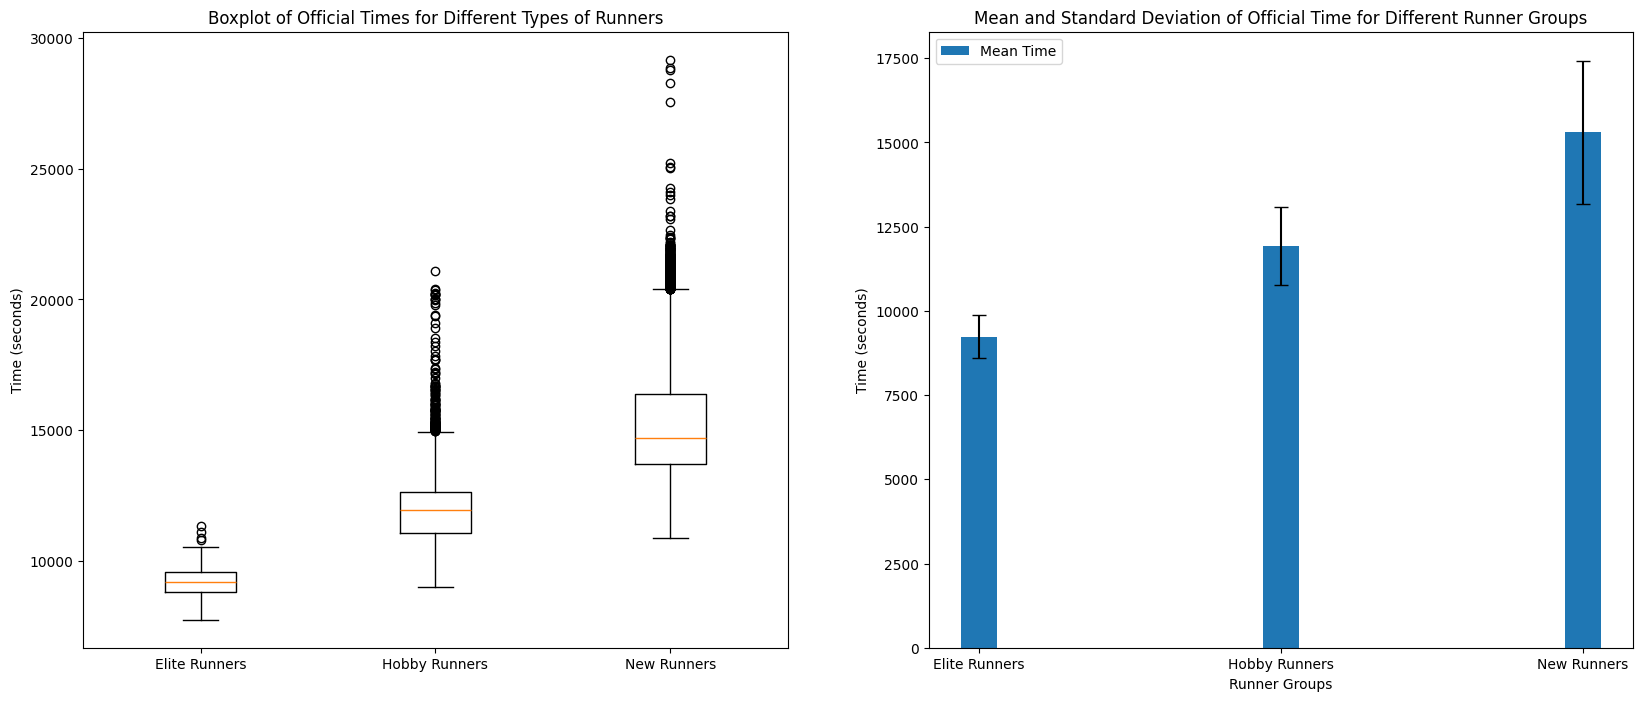
\includegraphics[width=\linewidth]{figs/elite_hobby_new_standar_deviation.png}}
    \caption{Standard deviation of race times for elite, hobby, and new runners.}
    \label{fig:elite_hobby_new_standar_deviation}
\end{figure}

\begin{figure}[htbp]
    \centerline{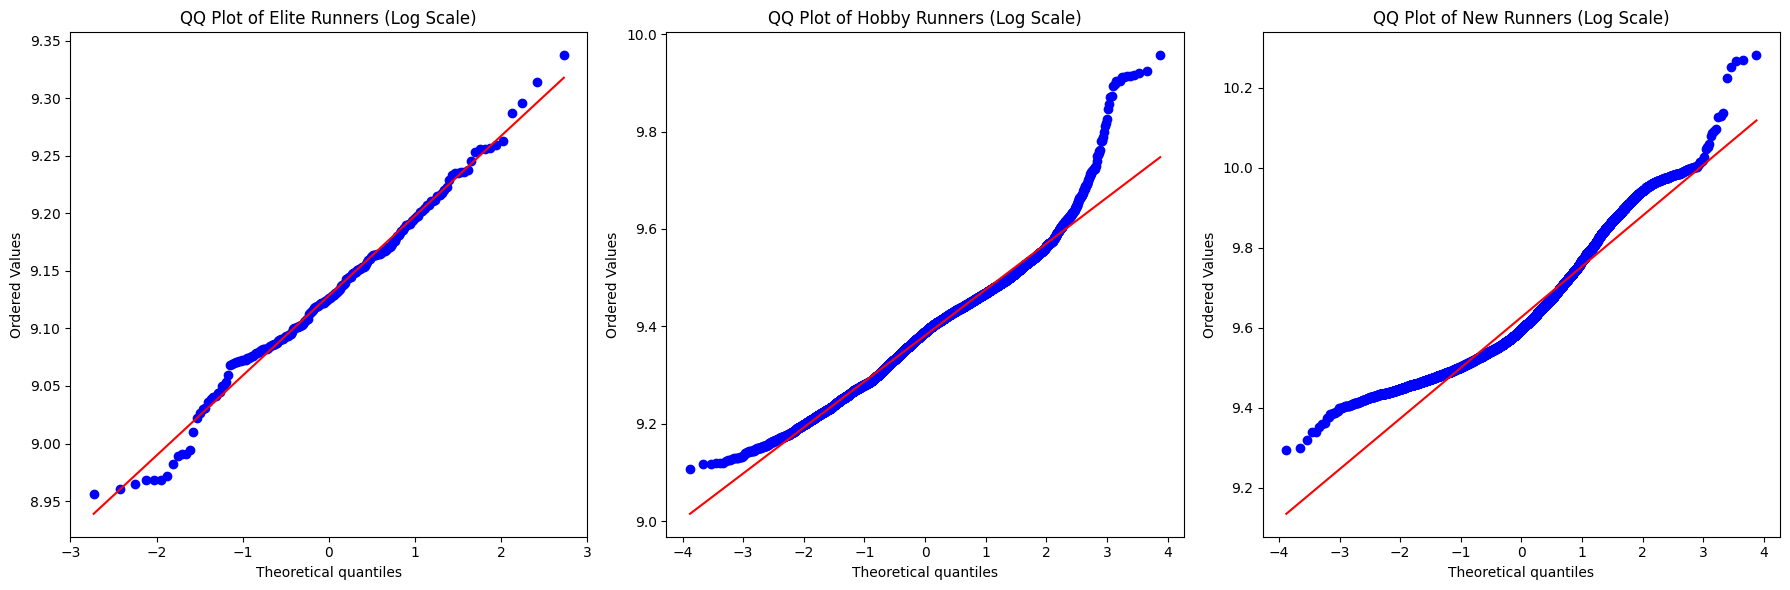
\includegraphics[width=\linewidth]{figs/elite_hobby_new_qq.png}}
    \caption{Q-Q plot for new runners.}
    \label{fig:new_qq}
\end{figure}

\section{Coding}
\subsection{Data}
\section{Definition of the experimental framework}
\section{Model validation}
\section{Results/Conclusions}

\begin{thebibliography}{00}
% \bibitem{b1} G. Eason, B. Noble, and I. N. Sneddon, ``On certain integrals of Lipschitz-Hankel type involving products of Bessel functions,'' Phil. Trans. Roy. Soc. London, vol. A247, pp. 529--551, April 1955.
% \bibitem{b2} J. Clerk Maxwell, A Treatise on Electricity and Magnetism, 3rd ed., vol. 2. Oxford: Clarendon, 1892, pp.68--73.
% \bibitem{b3} I. S. Jacobs and C. P. Bean, ``Fine particles, thin films and exchange anisotropy,'' in Magnetism, vol. III, G. T. Rado and H. Suhl, Eds. New York: Academic, 1963, pp. 271--350.
% \bibitem{b4} K. Elissa, ``Title of paper if known,'' unpublished.
% \bibitem{b5} R. Nicole, ``Title of paper with only first word capitalized,'' J. Name Stand. Abbrev., in press.
% \bibitem{b6} Y. Yorozu, M. Hirano, K. Oka, and Y. Tagawa, ``Electron spectroscopy studies on magneto-optical media and plastic substrate interface,'' IEEE Transl. J. Magn. Japan, vol. 2, pp. 740--741, August 1987 [Digests 9th Annual Conf. Magnetics Japan, p. 301, 1982].
% \bibitem{b7} M. Young, The Technical Writer's Handbook. Mill Valley, CA: University Science, 1989.
\bibitem{b8} B. Knechtle, C. McGrath, O. Goncerz, E. Villiger, P. T. Nikolaidis, T. Marcin, and C. V. Sousa, ``The Role of Environmental Conditions on Master Marathon Running Performance in 1,280,557 Finishers the ‘New York City Marathon’ From 1970 to 2019,'' Frontiers in Physiology, vol. 12, 2021. [Online]. Available: https://www.frontiersin.org/journals/physiology/articles/10.3389/fphys.2021.665761. DOI: 10.3389/fphys.2021.665761. ISSN: 1664-042X.


\end{thebibliography}
\vspace{12pt}

\end{document}
